\setminted{fontsize=\normalsize,baselinestretch=1}

\begin{frame}[fragile,plain]{}
\includegraphics[page=2]{pipeline}
\begin{minted}{haskell}
newtype Fix (syn :: (* -> *) -> (* -> *)) (a :: *) where 
  In :: syn (Fix syn) a -> Fix syn a

newtype Parser a = Parser (Fix ParserF a)
data ParserF (k :: * -> *) (a :: *) where
  Pure :: a -> ParserF k a
  Satisfy :: (Char -> Bool) -> ParserF k Char
  Try :: k a -> ParserF k a
  Look :: k a -> ParserF k a
  NegLook :: k () -> ParserF k ()
  Empty :: ParserF k a
  Branch :: k (Either x y) -> k (x -> a) -> k (y -> a) -> ParserF k a
  (:<*>:) :: k (a -> b) -> k a -> ParserF k b
  (:*>:) :: k a -> k b -> ParserF k b
  (:<*:) :: k a -> k b -> ParserF k a
  (:<|>:) :: k a -> k a -> ParserF k a
\end{minted}
\end{frame}




\begin{frame}[fragile]{High level optimizer. Пример 1}
%\includegraphics[page=3]{pipeline}

\begin{minted}{haskell}
string :: String -> Parser String
string = traverse char
\end{minted}

\begin{minted}{haskell}
string "ab"
-- urolling
pure (:) <*> char 'a' <*> (pure (:) <*> char 'b' <*> pure [])
-- Applicative fusion optimizations ....
satisfy (== 'a') *> satisfy (== 'b') *> pure "ab"
\end{minted}

\begin{block}{Законы аппликативов}
\lawApp
\end{block}
\end{frame}




%\defverbatim[colored]{\haskellOptZero}{
%\begin{lstlisting}[language=haskell,mathescape=false]
%      (f <$> p) <*> (g <$> q)
%=> 
%      (\x y -> (f x) (g y)) <$> p <*> q
%\end{lstlisting}
%}

%\defverbatim[colored]{\haskellOptOne}{
%\begin{lstlisting}[language=haskell,mathescape=false]
%      string "ab"
%      = 
%      char 'a' <:> char 'b' <:> pure []
%=>
%      satisfy (== 'a') *> satisfy (== 'b') $> "ab"
%\end{lstlisting}
%}

%\defverbatim[colored]{\haskellOptTwo}{
%\begin{minted}{haskell}
%string "ab"   ===   char 'a' <:> char 'b' <:> pure []
%\end{minted}      
%}
%\defverbatim[colored]{\haskellOptThree}{
%\mintinline{haskell}{satisfy (== 'a') *> satisfy (== 'b') $> "ab" }
%}


\setminted{fontsize=\Large,baselinestretch=1}

\begin{frame}[fragile]{High level optimizer. Пример 2}
%\includegraphics[page=3]{pipeline}

\begin{center}
\mintinline{haskell}{ (f <$> p) <*> (g <$> q) } 

\newln 
{\Huge $\Downarrow$} \newln 

\mintinline{haskell}{(\x y -> (f x) (g y)) <$> p <*> q }

\end{center}

\newln 

\Large Сэкономили одну операцию
\end{frame}

\begin{frame}[fragile]{High level optimizer. Пример 3}
%\includegraphics[page=3]{pipeline}
\begin{lstlisting}[language=haskell]
ident :: String -> Maybe String
ident = some (oneOf ['a' .. 'z']) `filteredBy` (not . isKeyword)
\end{lstlisting}
Превращается в более эффективный
\begin{lstlisting}[language=haskell]
ident input =
  let loop (c : cs) dxs finish | isAlpha c = loop cs (dxs . (c:)) finish
      loop cs dxs finish = finish (dxs []) cs
  in case input of
    c : cs | isAlpha c -> loop cs id ( λ xs _ -> if isKeyword (c:xs)
                                                   then Nothing 
                                                   else Just (c:xs))
    _ ->  Nothing
\end{lstlisting}
\end{frame}


%%%%%%%%%%%%%%%%%%%%%%%%%%%%%%%%%%%%%%%%%%%%%%%%%%%%%%%%%%%%%%%%%%%%%


%\setminted{fontsize=\normalsize,baselinestretch=1}



\setminted{fontsize=\Large,baselinestretch=1}
\defverbatim[colored]{\haskellLetZero}{
\begin{minted}{haskell}
many :: Parser a -> Parser a 
many p = (p <:> many p) <|> (pure p)
\end{minted}
}

\defverbatim[colored]{\haskellLetOne}{
\begin{minted}{haskell}
many :: Parser a -> Parser [a]
many p = 
  let go = (p <:> go) <|> (pure p) 
  go 
\end{minted}
}
\setminted{fontsize=\normalsize,baselinestretch=1}

\begin{frame}{High level optimizer. Борьба с рекурсией -- вставка let}
%\includegraphics[page=3]{pipeline}
\newln

\Large Исходный вариант:
\haskellLetZero

\newln 

Оптимизированный вариант:
\haskellLetOne
\end{frame}


\begin{frame}{High level optimizer. Больше анализов}
\includegraphics[page=3]{pipeline}
\newln 

\large 
\begin{itemize}
\item Consumption (<<поглощения>>) + cut (<<отсечения>>)
\begin{itemize}\large 
\item Consumption -- сколько символов <<поедает>> парсер
\item Cut нужны для более адекватных сообщениях об ошибках
\item Вставка правильных "отсечений" может быть нетривиальна
\end{itemize}
\newln 

\item Termination
\begin{itemize}\large 
\item Анализ точный для КС-грамматик и полностью аппликативных парсеров
\item В остальных случаях анализ неточный и ложные срабатывания игнорируются
\end{itemize}
\end{itemize}
\end{frame}




\begin{frame}[fragile]{Абстрактная машина}
\begin{itemize}
\item CPS 
\item Нужен стек, так как нет монад, но хочется КЗ
\end{itemize}
%Сказать про CPS, и так как у нас нет монады и КЗ, то обходимся стековой машиной
\newln

\begin{minted}{haskell}
data M (k :: [*] -> * -> * -> *) (xs :: [*]) (r :: *) (a :: *) where
  Halt :: M k [a] Void a
  Push :: x -> k (x : xs) r a -> M k xs r a
  Pop  :: k xs r a -> M k (x : xs) r a
  ...
\end{minted}

\begin{itemize}
\item \mintinline{haskell}{k} -- дерево из комбинаторов (обычно \mintinline{haskell}{Fix M});
\item \mintinline{haskell}{xs} --  type-level список, хранит типы значений на стеке перед исполнением инструкции;
\item \mintinline{haskell}{r} -- это тип возвращаемого машиной значения (полезно для рекурсии);
\item \mintinline{haskell}{a} -- тип финального результата парсинга, соответствует типы исходного парсера на комбинаторах.

\end{itemize}
\end{frame}


\begin{frame}[fragile]{Компиляция (1/6). Операции со стеком}
\begin{minted}{haskell}
compile :: Fix ParserF a -> Fix M [] Void a
compile = cata compAlg halt

type CodeGen a x = forall xs r . Fix M (x : xs) r a -> Fix M xs r a

compAlg :: ParserF (CodeGen a) x -> Fix M (x : xs) r a -> Fix M xs r a
compAlg (Pure x) = push x
compAlg (p :*>: q) = p . pop . q
compAlg (p :<*: q) = p . q . pop
\end{minted}
\end{frame}

\begin{frame}[fragile]{Компиляция (2/6). Аппликативы}
\begin{minted}{haskell}
data M (k :: [*] -> * -> * -> *) (xs :: [*]) (r :: *) (a :: *) where
  ...
  Lift2 :: (x -> y -> z) -> k (z : xs) r a -> M k (y : x : xs) r a
  Swap :: k (x : y : xs) r a -> M k (y : x : xs) r a
  
app = lift2 id
compAlg :: ParserF (CodeGen a) x -> Fix M (x : xs) r a -> Fix M xs r a
compAlg (pf :<*>: px) = pf . px . app

\end{minted}
\end{frame}

\begin{frame}[fragile]{Компиляция (3/6). Selectives }
\begin{minted}[escapeinside=!!]{haskell}
data M (k :: [*] -> * -> * -> *) (xs :: [*]) (r :: *) (a :: *) where
  ...
  Case :: k (x : xs) r a -> k (y : xs) r a -> M k (Either x y : xs) r a
  
compAlg :: ParserF (CodeGen a) x -> Fix M (x : xs) r a -> Fix M xs r a  
compAlg (Branch b l r) = λk -> 
  b (!case! (l (swap (app k))) (r (swap (app k))))
\end{minted}
\newln 

\begin{itemize}
\item Запускаем b
\item В продолжении проверяем с помощью \verb=case= на \mintinline{haskell}{Left/Right}
\item В зависимости от результата запускаем \mintinline{haskell}{l}
или \mintinline{haskell}{r} вместе с \mintinline{haskell}{k}
\end{itemize}
\end{frame}

\begin{frame}[fragile]{Компиляция (4/6). Alternatives}
%TODO: рассказать про две реализации alternative выше
%TODO: сказать про второй стек
Функции \mintinline{haskell}{catch,handle,commit} для работы со стеком, где лежат \emph{handlers}...

\begin{minted}[escapeinside=!!]{haskell}
data M (k :: [*] -> * -> * -> *) (xs :: [*]) (r :: *) (a :: *) where
  ...
  Fail :: M k xs r a
  Catch :: k xs r a -> k (String : xs) r a -> M k xs r a
  Commit :: k xs r a -> M k xs r a
  
handle :: (Fix M xs r a -> Fix M (x : xs) r a) -> Fix M (String : xs) r a
  -> Fix M (x : xs) r a -> Fix M xs r a
handle p h k = catch (p (commit k)) h

compAlg :: ParserF (CodeGen a) x -> Fix M (x : xs) r a -> Fix M xs r a
compAlg (p :<|>: q) = λk -> handle p (parsecHandle (q k)) k
compAlg Empty = const fail
...
\end{minted}
\end{frame}



\begin{frame}[fragile]{Компиляция (5/6). Примитивные инструкции}
\begin{minted}{haskell}
data M k (xs :: [*]) r a where
  ...
  Sat :: (Char -> Bool) -> k (Char : xs) r a -> M k xs r a
  Tell :: k (String : xs) r a -> M k xs r a
  Seek :: k xs r a -> M (String : xs) r a
  Ret :: M k [r] r a
  Call :: MuVar x -> k (x : xs) r a -> M k xs r a

compAlg (Satisfy p) = sat p
compAlg (Try p) = handle p (seek fail)
compAlg (Look p) = tell . p . swap . seek
compAlg (Let _ μ) = call μ
\end{minted}
\newln 

\begin{itemize}
\item \mintinline{haskell}{tell} кладет вход на стек
\item \mintinline{haskell}{seek} возвращает в исходное состояние
\end{itemize}
\end{frame}

%\begin{comment}
\begin{frame}[fragile]{Компиляция (6/6). Negative lookahead}
\begin{minted}{haskell}
negLook p = try (look p *> empty) <|> pure ()

\end{minted}
\pause 
\newln 

А вот так правильно
\begin{minted}{haskell}
negLookM p = join (try (look p *> pure empty) <|> pure (pure ()))
\end{minted}
\newln 

Реализация в машине
\begin{minted}{haskell}
compAlg (NegLook p) = λk -> 
  handle (tell . p . pop . seek) (seek (push () k)) fail
\end{minted}
\end{frame}

%\end{comment}




\begin{frame}[fragile]{}
\includegraphics[page=5]{pipeline}
\begin{itemize}
\item Join points ($\varphi$-узлы) 
\begin{minted}{haskell}
compAlg (p :<|>: q) = λk -> handle p (parsecHandle (q k)) k
\end{minted}
Решается с помощью специальной инструкции машины \mintinline{haskell}{Join}, которая вставляется после 
\mintinline{haskell}{Case} и \mintinline{haskell}{Catch}
\item Хвостовая рекурсия
\begin{itemize}
\item Достигается введением инструкций \mintinline{haskell}{Jump} и \mintinline{haskell}{Call}
\end{itemize}
\item Deep inspection (via histomoprhism)
\begin{itemize}
\item Поиск различных шаблонов и их замена на более компактные операции
\end{itemize}
\end{itemize}

%\begin{itemize}
%\item Cut 
%\begin{itemize}
%\item TODO
%\end{itemize}
%\item Termination
%\begin{itemize}
%\item Анализ точный для КС-грамматик и наивных аппликатиных парсеров
%\item В остальных случаях анализ неточный и ложные срабатывания игнорируются
%\end{itemize}
%\end{itemize}
\end{frame}

\begin{frame}[fragile]{Consumption анализ, попытка 2}
%\subtitle{
Оценка снизу сколько символов "поедает" парсер:
%}
\begin{minted}{haskell}
inputConsumed :: Fix M -> Int
inputConsumed = cata alg where 
  alg :: M Int -> Int
  alg Halt = 0
  alg (Push _ k) = k
  alg (Sat _ k) = k + 1
  alg (Catch p q) = min p q
  alg (Call _ _) = 0                -- пессимистично
  alg (MkJoin φ b k) = b + k
  alg (Join φ)  = 0
  ...
\end{minted}

N.B. Типы упрощены для краткости
\end{frame}

\subsection{Staging}


\begin{frame}[fragile]{Staging}
\begin{figure}[ht]
\begin{subfigure}[t]{.59\textwidth}
Обычная функция возведения в степень
\begin{minted}{haskell}
power :: Nat -> (Int -> Int)
power 0 = λx -> 1
power n = λx -> x * power (n - 1) x
\end{minted}
Staged функция, где степень известна \emph{статически}, а основание -- динамически
\begin{minted}{haskell}
power_ :: Nat -> Code (Int -> Int)
power_ 0 = [| λx -> 1 |]
power_ n = [| λx -> x * $(power_ (n-1)) |]
\end{minted}
\end{subfigure}
\hspace{.1\textwidth}
\begin{subfigure}[t]{.29\textwidth}
Quoting vs. splicing 
\vspace{1em}

Если \verb=x :: a= то \verb=[|x|] :: Code a= 
\vspace{1em}

и если  \verb=qx :: Code a=, то \verb=$(qx) :: a=.

\end{subfigure}
\end{figure}
\begin{center}
\begin{minipage}{10cm}
\begin{minted}{haskell}
power5 = $(power_ 5)
       = $([| λx -> x * x * x * x * x * 1 |])
       = λx -> x * x * x * x * x * 1
\end{minted}
\end{minipage}
\end{center}
\end{frame}

%%%%%%%%%%%%%%%%%%%%%%%%%%%%%%%%%%%%%%%%%%%%%%%%%%%%%%%
\defverbatim[colored]{\StagingParsleyI}{
\begin{minted}{haskell}
--

nonzero :: Parser Char 
nonzero :: oneOf ['1'..'9']
digit :: Parser Char 
digit = char '0' <|> nonzero 
natural :: Parser Int 
natural =
       read <$> (nonzero <:> many digit)

ident :: Parser String
ident = satisfy (     isAlpha)
  <:> many (satisfy (     alphaNum))
\end{minted}
}
\defverbatim[colored]{\StagingParsleyII}{
\begin{minted}{haskell}
--
{-# OPTIONS_GHC -fplugin=LiftPlugin #-}
nonzero :: Parser Char 
nonzero :: oneOf ['1'..'9']
digit :: Parser Char 
digit = char '0' <|> nonzero 
natural :: Parser Int 
natural =
  code read <$> (nonzero <:> many digit)

ident :: Parser String
ident = satisfy (code isAlpha)
  <:> many (satisfy (code alphaNum))
\end{minted}
}

\begin{frame}[t]{Staging для парсер-комбинаторов (пример)}
\only<1>{
\StagingParsleyI
}
\only<2>{
\StagingParsleyII
}
\end{frame}
%%%%%%%%%%%%%%%%%%%%%%%%%%%%%%%%%%%%%%%%%%%%%%%%%%%%%%%

\begin{frame}[fragile]{Компиляция в абстрактную машину}
\begin{minted}{haskell}
type Eval xs r a = Γ xs r a -> Maybe a
eval :: Fix M [ ] Void a -> (String -> Maybe a)
eval m = λ input -> cata alg m (Γ input HNil [] (error "Empty call stack"))
  where
    alg :: M Eval xs r a -> Eval xs r a
    alg Halt = evalHalt
    alg (Push x k) = evalPush x k
    alg ...
    
data Γ xs r a = Γ 
    { input :: String, ops :: HList xs
    , hs :: [String -> Maybe a], retCont :: r -> String -> Maybe a }
data HList (xs :: [*]) where
  HNil :: HList []
  HCons :: x -> HList xs -> HList (x : xs)   
\end{minted}
\end{frame}


\begin{frame}[fragile]{Реализация машины (1/5)}
\begin{minted}{haskell}
type Eval' xs r a = Code (Γ xs r a -> Maybe a) 
eval' :: Fix M xs Void a -> Code (String -> Maybe a)
data Γ' xs r a = Γ'
  { input :: Code String , ops :: Code (HList xs)
  , hs :: Code [String -> Maybe a] , retCont :: Code (r -> String -> Maybe a) }
\end{minted}
\vspace{1em}
% Тут важное замечание на тему того, почему Code можно пропихнуть внутрь списка
\begin{minted}{haskell}
type Eval'' xs r a = Γ' xs r a -> Code (Maybe a)
data Γ'' xs r a = Γ'' 
  { input :: Code String, ops :: QList xs
  , hs :: [Code (String -> Maybe a) ]
  , retCont :: Code (r -> String -> Maybe a) }
data QList (xs :: [*]) where
  QNil :: QList [ ]
  QCons :: Code x -> QList xs -> QList (x : xs)
\end{minted}
\end{frame}



\begin{frame}[fragile]{Реализация машины (2/5)}
\begin{minted}{haskell}
eval :: Fix M [ ] Void a -> (String -> Maybe a)
eval m = λ input -> 
    cata alg m (Γ input HNil [] (error "Empty call stack"))
  where alg :: M Eval xs r a -> Eval xs r a
        alg Halt = evalHalt
        alg (Push x k) = evalPush x k
        alg ...

        evalHalt :: (Γ [a] Void a -> Maybe a)
        evalHalt = λγ -> let HCons x = ops γ in Just x

eval''' m = [| λ input -> 
    $(cata alg''' m (Γ''  [| input |] QNil [] [| noret |])) |]
  where ...
    evalHalt''' γ = let QCons qx = ops γ in [| Just $(qx) |]

\end{minted}

\end{frame}

\begin{frame}[fragile]{Реализация машины (3/5)}
\begin{minted}{haskell}
evalLift2 :: (x -> y -> z) -> Eval (z : xs) r a 
          -> (Γ (y : x : xs) r a -> Maybe a)
evalLift2 f k = λγ -> let HCons y (HCons x xs) = ops γ in 
                      k (γ { ops = HCons (f x y) xs })
\end{minted}
%The Lift2 instruction extracts the top two elements of the stack and uses its given function f to create a value of type z required on the stack for the partially evaluated continuation machine k.
\newln
\begin{minted}{haskell}
evalLift2''' qf k γ = 
  let QCons qy (QCons qx xs) = ops γ in 
  k (γ { ops = QCons [| ($(qf) $(qx) $(qy)) |] xs })
\end{minted}
% Again, the stack operations have been moved outside of the quotations: the elements of the stack are obtained at compile time. The only work performed in this instruction at run-time is the application f x y, even pushing this new value back onto the stack happens at compile time.

\end{frame}



\begin{frame}[fragile]{Реализация машины (4/5)}
\begin{minted}{haskell}
evalFail :: (Γ xs r a -> Maybe a)
evalFail = λγ -> case hs γ of 
                  h : [] -> h (input γ)
                  _      -> Nothing
\end{minted}
В случае ошибки пытаемся восстановиться первым попавшимся способом
\begin{minted}{haskell}
evalFail''' γ = case hs γ of 
  qh : [] -> [| $(qh) $(input γ) |]
  _       -> [| Nothing |]
\end{minted}
%The story for Fail is similar, establishing whether or not a failure handler exists is an operation
%performed at compile time: if one exists the instruction returns the code which corresponds to the
%application of this handler to the input otherwise returns code representing Nothing.
\end{frame}

\begin{frame}[fragile]{Реализация машины (5/5)}
\begin{minted}{haskell}
evalSat :: (Char -> Bool) -> Eval (Char : xs) r a -> (Γ xs r a -> Maybe a)
evalSat f k = λγ -> case input γ of
  c : cs | f c -> k (γ { input = cs, ops = HCons c (ops γ) })
  _            -> evalFail γ
\end{minted}
\vspace{2em}
Функция \mintinline{ocaml}{evalSat} -- \emph{полностью} динамическая, в отличие от предыдущих
\begin{minted}{haskell}
evalSat''' qf k γ = [| case $(input γ) of
  c : cs | $(qf) c -> $(k (γ { input = [|cs|], ops = QCons [|c|] (ops γ) }))
  _                -> $(evalEmpt γ) |]
\end{minted}
\end{frame}

\begin{comment}
%\begin{frame}[fragile]{Реализация машины (6/6)}
%\begin{minted}{haskell}
%negLook p = try (look p *> empty) <|> pure ()
%\end{minted}
% \pause 
%Это была неправильная реализация.
%
%А вот правильная
%\begin{minted}{haskell}
%negLookM p = join (try (look p *> pure empty) <|> pure (pure ()))
%\end{minted}
%\pause 
%\vspace{2em}
%Фишка в том, что кое-что непредставимое <<в лоб>> в комбинаторах, может быть представлено в машине 
%\begin{minted}{haskell}
%compAlg (NegLook p) = λk -> 
%  handle (tell . p . pop . seek) (seek (push () k)) fail
%\end{minted}
%\end{frame}
\end{comment}
